% This work is licensed under the Creative Commons
% Attribution-NonCommercial 3.0 Unported License. To view a copy of this
% license, visit http://creativecommons.org/licenses/by-nc/3.0/.

\section{Durchführung}

\subsection{Versuchsaufbau}

In diesem Versuch verwenden wir als Strahlenquelle ein Am-Präparat und
einen Halbleiter-Sperrschichtzähler als Detektor, wie bereits zuvor
erwähnt. Beide befinden sich in einem evakuierbaren Glaszylinder. Das
Präparat läßt sich horizontal verschieben. Die Stromimpulse des
Sperrschichtzählers werden durch einen Vorverstärker verstärkt und
anschließend von einem Vielkanalanalysator gezählt. Dabei wird auch ein
Energiespektrum der Stromimpulse erstellt. Mit dem Programm
\enquote{Multichannel Analyzer}~(MCA) wird der Vielkanalanalysator
angesprochen. In Abbildung~\ref{fig:schema-aufbau} ist ein Schema des
Aufbaus dargestellt.

\begin{figure}
  \centering
  \includegraphics{aufbau.pdf}
  \caption{Schema des Versuchsaufbaus}
  \label{fig:schema-aufbau}
\end{figure}

\subsection{Messung zur Reichweite der Strahlung}

Um die Reichweite der $\alpha$-Strahlung zu bestimmen, wird bei
festgelegtem Abstand zwischen Strahlenquelle und Detektor die Anzahl der
Stromimpulse bei verschiedenen Drü"-cken gemessen und das Maximum der
Energie abgelesen; Volumen und Temperatur bleiben dabei konstant. Es
wird pro Druck \SI{120}{\second} lang gemessen. Dabei wird mit einem
Druck von ca. \SI{0}{\milli\bar} begonnen und der Druck pro Messung um
\SI{50}{\milli\bar} erhöht, bis Normaldruck erreicht ist. Anschließend
wird die Messreihe mit einem veränderten Abstand zwischen Strahlenquelle
und Detektor erneut durchgeführt.  Mit Formel
\eqref{eq:effektive_laenge} lässt sich bei festem Abstand $x_0$ zwischen
Strahlenquelle und Detektor in Abhängigkeit vom Druck im Glaszylinder
eine effektive Länge $x$ angeben. Diese effektive Länge gibt an, wie
groß der Abstand zwischen Strahlenquelle und Detektor sein müsste, wenn
die Messung bei festem Atmosphärendruck $p_0$ durchgeführt würde, um ein
äquivalentes Verhalten der Anzahl der ankommenden $\alpha$-Teilchen zu
erhalten wie bei dem eingestelltem Druck $p$. Erst dadurch kann man also
die Reichweite der Teilchen durch Variation des Druckes bestimmen.

\begin{equation}
  \label{eq:effektive_laenge}
  x = x_0 \cdot \frac{p}{p_0}
\end{equation}

 
\subsection{Messung zur Statistik des radioaktiven Zerfalls}
Um die Zerfallsrate angeben zu können, wird für jeweils \SI{10}{\second}
die Anzahl der Stromimpulse gemessen. Dieser Vorgang wird 100mal
wiederholt, um eine statistische Aussage treffen zu können
